\documentclass{article}
\usepackage{ctex} % 支持中文
\usepackage{graphicx} % 插入图片
\usepackage{geometry} % 页面布局
\usepackage{titlesec} % 自定义标题样式
\usepackage{setspace} % 设置行距
\usepackage{fancyhdr} % 页眉页脚
\usepackage{zhnumber} % 中文数字包
\usepackage{float}
\usepackage{tocloft} % 控制目录样式

% 页面布局设置
\geometry{a4paper, left=2.5cm, right=2.5cm, top=2.0cm, bottom=2.0cm}  % 更紧凑的页面布局

% 设置字体
\setCJKmainfont{SimSun}  % 宋体
\setCJKsansfont{Microsoft YaHei}  % 微软雅黑

% 设置行距
\setlength{\parindent}{1.5em}  % 段落首行缩进
\setlength{\parskip}{0.3em}  % 段落间距
\onehalfspacing  % 1.5 倍行距

% 自定义标题样式
\titleformat{\section}
  {\normalfont\fontsize{14pt}{18pt}\bfseries\songti}{\thesection}{1em}{} % 一级标题(黑体三号加粗)
\titleformat{\subsection}
  {\normalfont\fontsize{12pt}{16pt}\bfseries\songti}{\thesubsection}{1em}{} % 二级标题(宋体小四号加粗)
\titleformat{\subsubsection}
  {\normalfont\fontsize{12pt}{16pt}\songti}{\thesubsubsection}{1em}{} % 三级标题(宋体小四号)

% 设置目录的样式
\renewcommand{\contentsname}{\centerline{\bfseries \LARGE 目录}} % 设置目录标题样式
\setlength{\cftbeforesecskip}{0.5em}  % 减少目录项之间的间距
\setlength{\cftbeforesubsecskip}{0.3em}  % 减少子目录项之间的间距

% 页眉页脚设置
\pagestyle{fancy}
\fancyfoot[C]{2025年4月} % 日期在页脚

\begin{document}

% 封面
\begin{titlepage}
    \centering
    \vspace*{0.5cm}  % 控制图片上方的空白间距
   
\includegraphics[width=0.5\textwidth]{images/logo.png}
    \\  % 图片路径
    \vspace{1.5cm} % 图片与标题之间的空白间距
    \textbf{\LARGE 基于预训练大模型的高保真三维智能\\驾驶场景生成系统} \\[1.5em]
    \begin{tabular}{@{}ll@{}}
        学生姓名 & 郑睿翔 \\[1em]
        学号 & 2123030045 \\[1em]
        学院 & 人工智能与先进计算学院 \\[1em]
        专业班级 & 数智2102 \\[1em]
        指导教师 & 王海东 \\[1em]
        职称 & 教授 \\[1em]
    \end{tabular}
    \vspace{2cm} % 学院信息与日期之间的空白间距
    \vfill  % 向下推送日期
    \begin{center}
        2025年4月
    \end{center}
\end{titlepage}

\newpage
% 原创性声明页面
\begin{titlepage}
    \centering
    \vspace*{2cm}
    \textbf{\LARGE 湖南工商大学本科毕业论文(设计)原创性声明}\\[2em]
    本人郑重声明:所呈交的本科毕业论文(设计)是本人在指导老师的指导下,独立进行研究工作所取得的成果,成果不存在知识产权争议,除文中已经注明引用的内容外,本论文(设计)不含任何其他个人或集体已经发表或撰写过的作品成果。对本文的研究做出重要贡献的个人和集体均已在文中以明确方式标明。本人完全意识到本声明的法律结果由本人承担。\\[2em]
    作者签名:郑睿翔\\[1em]
    日期:2025年4月11日
\end{titlepage}

% 知识产权及使用授权声明书页面
\newpage
\begin{titlepage}
    \centering
    \vspace*{2cm}
    \textbf{\LARGE 湖南工商大学本科毕业论文(设计)知识产权及使用授权声明书}\\[2em]
   本毕业论文(设计)《基于预训练大模型的高保真三维智能驾驶场景生成系统》是本人在校期间所完成学业的组成部分,是在学校教师的指导下完成的。因此,本人特授权学校可将本毕业论文(设计)的全部或部分内容编入有关书籍、数据库保存,可采用复制、印刷、网页制作等方式将论文(设计)文本和经过编辑、批注等处理的论文(设计)文本提供给读者查阅、参考,可向有关学术部门和国家有关教育主管部门呈送复印件和电子文档。本毕业论文(设计)无论做何种处理,必须尊重本人的著作权,署明本人姓名。\\[2em]
    论文(设计)作者(签字)郑睿翔
    时间2025年4月11日\\
    指导教师已阅(签字)时间年月日
    \\[1em]
\end{titlepage}

\newpage
% 目录
\tableofcontents

\newpage

% 摘要页面
\begin{titlepage}
    \centering
    \textbf{\LARGE 摘\quad 要}\\[2em]
    智能驾驶测试场景构建效率低下是当前行业面临的重要问题。为此,本文提出了一种融合大语言模型(LLM)与形式化场景描述语言的新型生成框架,旨在高效地将自然语言描述转化为高保真三维测试场景。该框架包含三大核心模块:一是领域知识增强的指令解析模块,能够精准理解自然语言描述中的测试场景需求,为后续生成工作奠定基础;二是语法 - 语义双验证代码生成机制,确保生成的Scenic代码不仅语法正确,还符合实际场景的语义逻辑,从而提高代码的可用性和准确性;三是物理规则驱动的场景合成引擎,依据物理规则合理生成三维场景,保证场景的真实性和可靠性。在CARLA仿真平台的实验验证中,该系统展现出优异的性能:生成的Scenic代码准确率高达92.3%,场景物理合规率超过85%,且生成时延低于3秒/场景。这一成果显著提升了智能驾驶测试场景的构建效率,为智能驾驶技术的测试与优化提供了高效、准确的工具支持,有望推动智能驾驶领域相关测试工作的高效开展,促进智能驾驶技术的进一步发展与完善,具有重要的应用价值和广阔的发展前景。\\[2em]
    \textbf{关键词:} 智能驾驶;测试场景;大语言模型;Scenic代码;CARLA仿真;生成框架
\end{titlepage}
% 第一章 绪论
\section{绪论}
\subsection{研究背景}
\subsubsection{智能驾驶测试对海量长尾场景的需求矛盾}
随着智能驾驶技术的飞速发展,其测试需求也日益复杂和多样化。智能驾驶系统需要在各种复杂多变的交通场景下表现出可靠的性能,以确保驾驶的安全性和舒适性。然而,现实交通环境中存在着海量的长尾场景,这些场景虽然出现频率较低,但一旦发生,往往会对智能驾驶系统构成严峻挑战。
长尾场景的复杂性主要体现在以下几个方面。首先,交通环境的动态性极强,车辆、行人、非机动车等多种交通参与者的行为模式千变万化。例如,在城市道路中,行人可能会突然横穿马路,非机动车可能会随意变道或逆行,这些行为都可能导致潜在的碰撞风险。智能驾驶系统必须能够准确感知和预测这些行为,并做出合理的决策。其次,道路条件的多样性也增加了测试场景的复杂性。从城市快速路到乡村小道,从高速公路到山区道路,不同道路的几何形状、路面状况、交通标志和信号灯等都有所不同。智能驾驶系统需要在这些不同的道路条件下都能正常运行。此外,天气条件和光照条件的变化也会对智能驾驶系统的感知和决策产生影响。雨、雪、雾等恶劣天气会降低传感器的性能,而不同的光照条件(如强光、弱光、逆光等)会影响视觉系统的识别效果。
为了确保智能驾驶系统的安全性和可靠性,测试过程中需要覆盖尽可能多的长尾场景。然而,这面临着巨大的挑战。一方面,长尾场景的数量庞大,几乎无法穷尽。要完全覆盖所有可能的场景几乎是不可能的任务。另一方面,这些场景的出现频率较低,难以在实际道路测试中频繁遇到。因此,传统的测试方法往往难以满足智能驾驶系统对海量长尾场景的测试需求,导致测试的充分性和有效性受到限制。

\subsubsection{传统场景构建方法的人力成本与效率瓶颈}
在智能驾驶测试领域,传统的场景构建方法主要依赖于人工设计和开发。这些方法虽然在一定程度上能够满足测试需求,但也存在着显著的局限性。
首先,人工设计场景需要大量的专业人员投入。这些人员需要具备深厚的交通工程、计算机科学和智能驾驶技术等多学科知识,能够准确理解和模拟各种复杂的交通场景。然而,这样的人才相对稀缺,培养成本高昂。而且,随着测试需求的不断增加,对专业人员的需求也在持续增长,这进一步加剧了人力成本的压力。
其次,人工设计场景的效率较低。设计一个复杂的交通场景需要经过需求分析、场景建模、代码编写和调试等多个步骤。每个步骤都需要耗费大量的时间和精力。例如,在场景建模阶段,需要精确地定义道路的几何形状、交通参与者的初始位置和行为模式等。在代码编写阶段,需要将这些模型转化为可执行的代码,这不仅需要专业的编程技能,还需要反复调试以确保代码的正确性和稳定性。因此,人工设计场景的速度远远无法满足智能驾驶系统快速迭代和测试的需求。
此外,人工设计场景的准确性和一致性也难以保证。由于不同设计人员的理解和经验不同,可能会导致设计出的场景存在差异。而且,在复杂的场景中,人工设计容易遗漏一些关键的细节,从而影响测试结果的准确性和可靠性。

\subsubsection{大语言模型在代码生成领域的突破性进展}
近年来,大语言模型(LLM)在自然语言处理领域取得了巨大的突破,并逐渐拓展到代码生成等领域。大语言模型通过在海量文本数据上进行预训练,学习到了语言的语法、语义和逻辑结构,能够生成自然流畅且符合逻辑的文本内容。这种能力为解决智能驾驶测试场景构建的难题提供了新的思路。
在代码生成领域,大语言模型已经展现出了强大的能力。通过对代码数据的学习,大语言模型能够理解代码的结构和逻辑,生成符合语法规范的代码片段。例如,一些基于大语言模型的代码生成工具可以根据用户输入的自然语言描述,自动生成相应的代码实现。这些工具已经在软件开发领域得到了广泛的应用,显著提高了代码开发的效率和质量。
大语言模型在代码生成中的优势主要体现在以下几个方面。首先,它能够快速生成代码,大大缩短了开发周期。传统的人工编写代码需要经过需求分析、设计、编码和调试等多个阶段,每个阶段都需要耗费大量的时间。而大语言模型可以根据输入的描述直接生成代码,减少了中间环节,提高了开发效率。其次,大语言模型生成的代码质量较高。它能够学习到代码的最佳实践和规范,生成的代码不仅符合语法规范,还具有良好的可读性和可维护性。此外,大语言模型还能够根据不同的需求生成多样化的代码实现,为开发者提供了更多的选择。
将大语言模型应用于智能驾驶测试场景构建,可以充分利用其在代码生成领域的优势,解决传统方法面临的困境。通过将自然语言描述的测试场景需求转化为代码实现,大语言模型可以快速生成高保真的测试场景,提高场景构建的效率和质量。同时,结合智能驾驶领域的专业知识,还可以进一步优化大语言模型的性能,使其更好地适应智能驾驶测试场景构建的需求。


\subsection{研究现状}
\subsubsection{自然语言到形式化描述转换技术(NL2Formal)}
自然语言到形式化描述转换技术(NL2Formal)是自然语言处理(NLP)领域的一个重要研究方向,其目标是将自然语言描述的意图或需求转化为精确的形式化语言,以便计算机能够理解和执行。在自动驾驶测试场景生成中,NL2Formal技术尤为重要,因为它可以将测试工程师的自然语言描述转化为精确的测试场景代码,从而提高测试效率和准确性。早期的NL2Formal技术主要基于规则,通过预定义的规则或语义解析器来理解自然语言查询并将其转换为形式化语言。这种方法的优点是规则明确,易于理解和实现,但缺点是灵活性差,难以处理复杂的自然语言现象。随着神经网络技术的发展,基于神经网络的方法逐渐成为主流。序列到序列模型和图神经网络被广泛应用于自然语言到SQL查询的转换任务中,取得了显著的进展。这些方法通过学习自然语言和形式化语言之间的映射关系,能够生成更准确的形式化代码。近年来,预训练语言模型(如BERT和T5)的出现进一步推动了NL2Formal技术的发展。这些模型通过在大规模文本数据上进行预训练,学习到了语言的语法、语义和逻辑结构,能够生成高质量的形式化语言。最新的研究则进入了大型语言模型(LLMs)时代,LLMs具有卓越的语言理解和生成能力,可以通过提示(prompting)技术执行NL2Formal任务,生成高质量的形式化代码。这些技术的不断发展和应用,为自动驾驶测试场景的高效生成提供了新的可能性。

\subsubsection{Scenic语言在自动驾驶仿真中的应用}
Scenic是一种用于自动驾驶仿真测试的形式化场景描述语言,它允许测试工程师以简洁、直观的方式描述复杂的交通场景。Scenic语言的核心优势在于其强大的表达能力和灵活性,能够精确地定义交通参与者的初始位置、行为模式以及环境条件。在自动驾驶仿真中,Scenic语言的应用主要体现在场景建模、代码生成和场景合成等方面。通过Scenic语言,测试工程师可以定义车辆的初始位置、速度、加速度以及行人横穿马路的行为模式,从而构建出高度复杂的交通场景。Scenic语言的代码生成机制能够将场景描述转化为可执行的仿真代码,这使得测试工程师可以专注于场景的逻辑设计,而无需关心底层的代码实现。此外,Scenic语言支持场景的合成和组合,可以将多个简单的场景组合成复杂的场景,大大提高了场景生成的效率,同时也保证了场景的多样性和复杂性。Scenic语言的这些特性使其在自动驾驶仿真测试中得到了广泛应用,成为自动驾驶测试领域的重要工具之一。

\subsubsection{场景生成质量评估方法研究进展}
场景生成质量评估是自动驾驶测试中的一个重要环节,它直接影响到测试结果的可靠性和有效性。近年来,随着自动驾驶技术的发展,场景生成质量评估方法也取得了显著进展。目前,场景生成质量评估方法主要集中在功能质量、美学质量和人因质量等方面。功能质量评估从场景物件的使用性与功能关联出发,通过可达性、可见性、开阔度、关联关系和功能比例等指标来衡量场景的功能质量。美学质量评估则基于场景平面构图和人视点视野,使用平衡性、齐整度与和谐性等指标来度量场景的美学质量。人因质量评估根据人类活动模拟,采用流线合理性和活动舒适度等指标评估人因质量。这些评估方法从不同角度对场景生成质量进行了全面的评估,为自动驾驶测试场景的优化提供了重要的参考。除了上述评估指标,还有一些研究提出了基于深度学习的评估方法。通过构建深度神经网络模型,自动学习场景生成质量的评估标准,这些方法能够自动识别场景中的问题,并提供优化建议。这些技术的不断发展和应用,为自动驾驶测试场景的高效生成和质量评估提供了重要的技术支持,未来有望进一步提高自动驾驶测试的效率和可靠性。


\subsection{研究内容}
\subsubsection{面向场景描述的领域知识图谱构建}
在自动驾驶测试场景生成中,构建面向场景描述的领域知识图谱是实现高效、准确场景生成的基础。领域知识图谱通过整合自动驾驶领域的专业知识,包括交通规则、道路类型、车辆行为模式、传感器特性等,为自然语言描述的解析和形式化代码的生成提供丰富的上下文信息和语义支持。
领域知识图谱的构建涉及多个关键步骤。首先,需要对自动驾驶领域的知识进行系统梳理和分类,明确知识的层次结构和关联关系。这包括对交通场景中的实体(如车辆、行人、道路、交通标志等)及其属性(如位置、速度、类型等)的定义,以及这些实体之间的关系(如车辆与道路的交互、车辆与行人的避让等)。通过构建知识图谱,可以将这些复杂的知识结构化地表示出来,便于后续的查询和推理。
在知识图谱的构建过程中,还需要考虑知识的动态更新和扩展。自动驾驶技术不断发展,新的交通规则、车辆类型和传感器技术等不断涌现,因此知识图谱需要具备良好的可扩展性和可更新性。通过持续的知识更新,可以确保知识图谱始终保持最新状态,从而为场景生成提供准确的知识支持。
此外,领域知识图谱的构建还需要考虑知识的表达和存储方式。知识图谱通常以图的形式存储,其中节点表示实体,边表示实体之间的关系。这种结构化的存储方式不仅便于知识的查询和推理,还能够支持复杂的知识融合和关联分析。通过知识图谱的构建,可以实现对自动驾驶场景描述的深度理解和语义解析,为后续的代码生成和场景合成提供坚实的基础。

\subsubsection{基于LLM的语义约束代码生成方法}
基于大型语言模型(LLM)的语义约束代码生成方法是实现自动驾驶测试场景高效生成的关键技术之一。LLM具有强大的语言理解和生成能力,能够根据自然语言描述生成高质量的形式化代码。然而,为了确保生成代码的准确性和可靠性,需要在代码生成过程中引入语义约束机制。
语义约束代码生成方法的核心在于将自然语言描述的语义信息转化为代码生成的约束条件。这些约束条件可以包括交通规则、道路类型、车辆行为模式等,确保生成的代码不仅符合语法规范,还满足实际场景的语义要求。通过语义约束机制,可以有效避免生成代码中的逻辑错误和不符合实际场景的情况,提高代码的质量和可用性。
在实现语义约束代码生成时,需要充分利用LLM的语言理解和生成能力。LLM可以通过对自然语言描述的深度理解,提取出关键的语义信息,并将其转化为代码生成的约束条件。同时,还需要开发相应的算法和工具,将这些约束条件嵌入到代码生成过程中,确保生成的代码能够准确地反映自然语言描述的语义内容。
此外,语义约束代码生成方法还需要考虑代码的可读性和可维护性。生成的代码不仅需要符合语法和语义规范,还需要具有良好的结构和注释,便于后续的修改和扩展。通过基于LLM的语义约束代码生成方法,可以实现从自然语言描述到形式化代码的高效转换,为自动驾驶测试场景的生成提供强大的技术支持。

\subsubsection{场景物理合理性的多模态验证机制}
场景物理合理性的验证是自动驾驶测试场景生成中的一个重要环节,它直接影响到测试场景的真实性和可靠性。为了确保生成场景的物理合理性,需要建立一种多模态验证机制,通过多种方式对场景进行综合验证。
多模态验证机制的核心在于结合多种验证手段,从不同角度对场景的物理合理性进行评估。这些验证手段可以包括基于物理规则的验证、基于仿真数据的验证以及基于专家知识的验证等。通过多种验证手段的结合,可以全面评估场景的物理合理性,确保生成的场景符合实际交通环境的物理规律。
基于物理规则的验证是多模态验证机制的重要组成部分。通过定义和应用物理规则,如牛顿运动定律、能量守恒定律等,可以对场景中的物体运动和交互进行验证。例如,可以验证车辆的加速度是否符合物理规律,车辆与行人之间的碰撞是否符合能量守恒等。这种基于物理规则的验证方法能够从理论上确保场景的物理合理性。
基于仿真数据的验证则是通过在仿真环境中运行生成的场景,收集仿真数据,并对数据进行分析和评估。通过对比仿真结果与实际交通数据,可以评估场景的物理合理性。例如,可以对比仿真中车辆的行驶速度、加速度等数据与实际交通数据的一致性。这种基于仿真数据的验证方法能够从实际运行的角度评估场景的物理合理性。
基于专家知识的验证则依赖于领域专家的经验和知识。通过邀请专家对生成的场景进行评估和审核,可以发现场景中可能存在的问题和不合理之处。专家可以根据自己的经验和知识,对场景中的车辆行为、交通规则遵守情况等进行评估,提出改进意见。这种基于专家知识的验证方法能够从实践经验和知识的角度评估场景的物理合理性。
通过建立场景物理合理性的多模态验证机制,可以全面评估生成场景的物理合理性,确保生成的场景符合实际交通环境的物理规律。这种多模态验证机制的建立,为自动驾驶测试场景的高质量生成提供了重要的保障,有助于提高自动驾驶测试的可靠性和有效性。





% 第二章 系统架构设计
\section{系统架构设计}
\subsection{整体架构}
在自动驾驶测试场景生成系统中,整体架构的设计是实现从自然语言描述到高保真三维测试场景端到端生成的关键。该架构通过多个紧密协同工作的模块,确保了系统的高效性、准确性和可靠性。系统的输入是自然语言描述的测试场景需求,这种描述方式使得测试工程师能够以直观、简洁的方式表达复杂的场景需求,无需深入技术细节。自然语言输入模块负责接收用户输入的文本描述,并将其传递到后续的处理模块。
接下来,自然语言输入被传递到自然语言处理(NLP)解析模块。该模块的核心任务是将自然语言描述转化为结构化的场景要素。NLP解析模块利用先进的自然语言处理技术,包括词法分析、句法分析和语义理解等,提取出描述中的关键信息。这些信息被进一步转化为场景要素的三元组形式,为后续的代码生成和场景合成提供基础。场景要素三元组以结构化的形式表示场景中的关键信息,每个三元组通常包含主体、关系和客体三个部分,这种结构化的表示方式能够清晰地描述场景中的实体及其相互关系。
随后,场景要素三元组被传递到语法验证器。语法验证器的作用是对NLP解析模块生成的场景要素三元组进行语法检查和验证。该模块通过预定义的语法规则,确保生成的三元组符合场景描述语言的规范。如果发现语法错误,语法验证器将触发修正机制,生成修正后的代码。修正代码模块负责根据语法验证器的反馈,对生成的代码进行修正和优化。该模块通过智能算法,自动识别和修复代码中的语法错误,同时优化代码的结构和性能。修正后的代码将被传递到场景合成引擎,用于生成具体的测试场景。
场景合成引擎是系统的核心模块之一,负责将修正后的代码转化为具体的三维测试场景。该模块结合物理规则和场景生成算法,生成高保真的三维场景。场景合成引擎不仅考虑场景的几何结构,还模拟了物理环境中的光照、天气和交通规则等因素,确保生成的场景具有高度的真实感和物理合理性。生成的三维场景随后被传递到三维可视化模块,该模块通过先进的图形渲染技术,将复杂的三维场景以直观的方式呈现给用户。用户可以通过交互式界面,观察和调整场景中的各种参数,进一步优化场景的生成效果。三维可视化不仅提高了场景的可理解性,还为用户提供了直观的反馈,便于对生成场景进行评估和调整。
最后,评估反馈系统对生成的三维场景进行质量评估和反馈。该模块通过一系列评估指标,包括场景的物理合理性、功能完整性和美学质量等,对生成的场景进行全面评估。评估结果将反馈给用户和系统,为后续的场景优化和系统改进提供依据。评估反馈系统不仅提高了场景生成的质量,还促进了系统的持续优化和改进。
整个系统通过各模块的紧密协同工作,实现了从自然语言描述到高保真三维测试场景的高效生成。在设计系统架构时,充分考虑了系统的扩展性和灵活性,使其能够适应不断变化的技术需求。随着自动驾驶技术的发展和测试需求的变化,系统能够方便地引入新的模块和功能,例如扩展NLP解析模块以支持更复杂的自然语言描述,或者在场景合成引擎中引入新的物理规则和算法,以生成更真实的测试场景。这种扩展性和灵活性使得系统能够保持其先进性和实用性。
系统的可靠性和稳定性是确保其在实际应用中有效运行的关键。通过在每个模块中引入错误处理和容错机制,系统能够有效地应对各种异常情况。例如,语法验证器可以识别并处理代码中的语法错误,修正代码模块能够自动修复这些问题,确保系统的稳定运行。此外,评估反馈系统通过持续的评估和反馈,进一步提高了系统的可靠性和稳定性。
为了提高系统的易用性,系统架构还注重用户友好性的设计。通过提供直观的交互界面和详细的用户指南,用户可以方便地输入自然语言描述,观察生成的三维场景,并根据评估反馈进行调整。这种用户友好的设计使得系统不仅适用于专业的测试工程师,还能够为非专业的用户提供支持,扩大了系统的应用范围。

\subsection{核心组件}
\subsubsection{自然语言处理模块}
自然语言处理(NLP)模块是自动驾驶测试场景生成系统的核心组成部分,其主要功能是将自然语言描述的测试场景需求转化为结构化的场景要素,为后续的代码生成和场景合成提供基础。自然语言处理模块的设计和实现涉及多个关键环节,包括领域专用词典构建方法、基于依存句法分析的三元组提取以及模糊指令的交互式澄清策略。这些环节共同确保了系统的高效性、准确性和可靠性。

\subsubsection{领域专用词典构建方法}
领域专用词典的构建是自然语言处理模块的基础,它为系统提供了与自动驾驶相关的专业术语和词汇,从而提高了系统对领域特定语言的理解能力。构建领域专用词典的过程可以分为语料库收集与预处理、词典构建与优化以及动态更新与扩展三个阶段。

语料库的收集与预处理是构建领域专用词典的第一步。这一过程需要收集大量与自动驾驶相关的文本数据,这些数据来源广泛,包括技术文档、用户手册、交通法规以及相关的新闻报道等。收集到的语料库需要经过预处理,包括文本清洗、分词以及标注等步骤。文本清洗的目的是去除无关字符和格式化文本,分词则是将文本分割成单词或短语,标注则是为每个单词或短语标注其词性。这些预处理步骤为后续的词典构建提供了高质量的数据基础。

词典的构建与优化是基于预处理后的语料库进行的。通过统计分析和机器学习方法,可以从语料库中提取领域专用词汇。例如,可以使用自然语言处理工具包(如NLTK)中的相关模块来管理和分析语料库。利用词频统计等技术,可以识别高频词汇,并将其纳入词典。为了进一步优化词典,可以采用词干提取和词形还原技术,将不同形式的单词归一化到其基本形式。这些技术有助于提高词典的准确性和一致性。

动态更新与扩展是领域专用词典的重要特性。随着自动驾驶技术的不断发展,新的术语和词汇不断涌现。因此,词典需要具备动态更新和扩展的能力,以反映最新的领域知识。可以通过定期收集新的语料库并重新训练词典,或者利用在线学习算法实时更新词典内容,从而确保词典始终处于最新状态。

\subsubsection{基于依存句法分析的三元组提取}
依存句法分析是自然语言处理中的一个重要任务,它通过分析句子中单词之间的依存关系来理解句子的结构和语义。在自动驾驶测试场景生成中,基于依存句法分析的三元组提取能够将自然语言描述转化为结构化的场景要素,从而为后续的代码生成提供准确的输入。

依存句法分析的目标是识别句子中单词之间的依存关系,例如主谓关系、动宾关系等。通过依存句法分析,可以构建出句子的依存树,从而清晰地展示单词之间的语义关系。依存句法分析的结果为三元组提取提供了基础,三元组通常以(主体,关系,客体)的形式表示,能够清晰地描述场景中的实体及其相互关系。这种结构化的表示方式为后续的代码生成提供了准确的输入。

为了提高三元组提取的准确性和效率,可以采用一些优化策略。例如,可以通过引入上下文信息和领域知识,对依存关系进行更准确的识别和分类。此外,还可以利用深度学习模型,如Transformer架构,来进一步提升依存句法分析的性能。这些优化策略有助于提高系统的准确性和效率,从而更好地满足自动驾驶测试场景生成的需求。

\subsubsection{模糊指令的交互式澄清策略}
在自动驾驶测试场景生成中,用户输入的自然语言描述可能存在模糊性或歧义。为了确保系统能够准确理解用户的需求,需要设计模糊指令的交互式澄清策略。这种策略通过与用户的交互,澄清模糊指令的含义,从而提高系统的准确性和可靠性。

模糊指令识别是交互式澄清策略的第一步。通过自然语言处理技术,如词性标注和依存句法分析,可以识别出用户输入中的模糊词汇或短语。这些技术能够帮助系统理解句子的结构和语义,从而识别出可能存在的模糊性。

交互式澄清是澄清模糊指令的关键环节。一旦识别出模糊指令,系统将与用户进行交互,通过提问或提供选项的方式澄清指令的含义。这种交互式澄清策略能够有效地减少模糊性,提高系统的理解能力。例如,系统可以询问用户关于模糊词汇的具体含义,或者提供一些预定义的选项供用户选择。通过这种方式,系统能够获得更准确的用户需求,从而生成更符合用户期望的测试场景。

用户反馈与学习是交互式澄清策略的重要组成部分。通过与用户的交互,系统不仅能够澄清模糊指令,还可以收集用户的反馈信息,从而进一步优化自然语言处理模块的性能。例如,可以根据用户的反馈调整词典内容、改进依存句法分析模型或优化澄清策略,以提高系统的准确性和用户体验。这种持续的学习和优化过程有助于系统不断改进,更好地满足用户的需求。

% 第三章 自然语言驱动的安全关键场景生成方法
\section{自然语言驱动的安全关键场景生成方法}
\subsection{基于检索增强的语义解析}
在自动驾驶系统开发与测试中,“安全关键场景”是指那些可能引发严重安全问题(如碰撞)的驾驶场景。为了确保自动驾驶车辆在复杂交通环境中的安全性,必须对这类场景进行充分的模拟与验证。因此,本研究明确将“安全关键场景”的量化标准设定为必须包含至少一个碰撞触发条件,如车辆或行人突然横穿道路、前方车辆急刹车等,这些条件直接关联到自动驾驶车辆可能面临的碰撞风险。
为了实现从自然语言指令到安全关键场景的高效转化,本研究采用基于检索增强的语义解析方法。自然语言指令中往往蕴含着对抗性成分,例如描述车辆或行人采取的突发性、干扰性行为。这些对抗性成分是生成安全关键场景的关键要素,需要准确解析并转化为符合 Scenic 语义规范的场景描述。Scenic 是一种专门用于描述自动驾驶场景的领域特定语言,能够以简洁、清晰的方式定义场景中各元素的行为与交互关系。通过对自然语言指令进行语义解析,提取其中的关键信息,并将其映射到 Scenic 的语言框架中,从而实现对安全关键场景的精确建模。
为了进一步提升语义解析的效率与准确性,本研究构建了一个向量化检索数据库。该数据库收录了大量经过标注与处理的场景描述及其对应的 Scenic 代码片段,形成了一个丰富的知识库。在解析新的自然语言指令时,系统首先将其转化为向量形式,然后在检索数据库中进行相似度匹配。通过设定相似度匹配阈值,系统能够快速筛选出与输入指令语义相近的已知场景描述,进而获取相应的 Scenic 代码片段作为参考或直接使用。这种方法不仅大大提高了语义解析的速度,还能够有效应对自然语言的多样性和复杂性,确保生成的场景代码的质量与可靠性。
基于预训练大模型的强大语言理解和生成能力,本研究的高保真三维智能驾驶场景生成系统能够高效地完成从自然语言指令到安全关键场景代码的转化。预训练大模型在海量文本数据上进行训练,具备了对自然语言的深刻理解以及生成高质量文本的能力。通过将预训练大模型与检索增强的语义解析方法相结合,系统能够在理解自然语言指令的基础上,快速检索到与之相关的场景知识,并生成符合 Scenic 语义规范的场景代码,从而实现对安全关键场景的高保真建模与生成。这一过程不仅充分利用了预训练大模型的语言优势,还通过检索数据库的辅助,进一步提升了场景生成的准确性和效率,为自动驾驶系统的安全测试与验证提供了有力支持。


\subsection{Scenic脚本生成技术}
Scenic脚本生成技术是自动驾驶场景生成中的关键技术,它通过灵活的语义规范和高效的代码片段融合算法,实现了从自然语言描述到可执行场景代码的高效转化。以下从“动态参数绑定”“多组件代码片段融合算法”“运行时语义校验机制”三个方面进行阐述。
\subsubsection{动态参数绑定与物理合规性}

Scenic语言通过“动态参数绑定”机制,确保生成的场景在物理上是合规的。在场景生成过程中,对象的属性(如位置、速度、加速度等)可能受到多种因素的约束。例如,车辆的最大加速度是一个重要的物理约束条件,它直接影响到车辆的运动轨迹和安全性。Scenic允许在定义对象时,通过“specifiers”(指定符)来动态绑定这些参数。这些指定符可以相互依赖,但语法上是独立的,Scenic会自动解析这些依赖关系,并按照正确的顺序进行评估。例如,当定义一个车辆的位置时,可以同时指定其模型(model),而模型的宽度又会影响车辆的位置计算。通过这种方式,Scenic能够在动态绑定参数的同时,确保所有参数都符合物理约束条件,从而保证生成的场景在物理上是合理的。
\subsubsection{多组件代码片段融合算法}
Scenic脚本生成技术中的多组件代码片段融合算法,是实现复杂场景生成的关键。在自动驾驶场景中,一个完整的场景可能由多个组件构成,如车辆、行人、道路、障碍物等。Scenic允许将这些组件分别定义为代码片段,然后通过融合算法将它们组合成一个完整的场景。这种融合算法不仅考虑了各个组件的属性和行为,还考虑了它们之间的相互关系。例如,在定义一个车辆时,可以单独定义其位置、速度、模型等属性,然后通过融合算法将这些属性组合在一起,形成一个完整的车辆对象。此外,Scenic还支持在融合过程中对组件进行随机化处理,从而生成多样化的场景。这种多组件代码片段融合算法大大提高了场景生成的灵活性和可扩展性,使得开发者能够轻松地定义和生成各种复杂的自动驾驶场景。
\subsubsection{运行时语义校验机制}
Scenic的运行时语义校验机制是确保生成场景质量的重要保障。在场景生成过程中,Scenic会自动对生成的场景进行语义校验,以确保场景的合理性和可行性。这种校验机制包括多个方面,如对象的可见性、对象之间的非交叉性、对象是否在指定区域内等。例如,Scenic会检查生成的车辆是否在道路上,车辆之间是否发生碰撞,以及车辆是否在视野范围内等。如果某个场景不满足这些语义条件,Scenic会自动重新生成场景,直到满足所有条件为止。此外,Scenic还允许用户定义自定义的语义校验规则,以满足特定场景的需求。这种运行时语义校验机制不仅提高了场景生成的可靠性,还减少了人工干预的需要,使得场景生成过程更加自动化和高效。

\subsection{生成效率优化}
\subsubsection{基于指令复杂度的自适应检索策略}
为了提高场景生成的效率,本研究提出了一种基于指令复杂度的自适应检索策略。在自动驾驶场景生成中,自然语言指令的复杂度直接影响到场景生成的难度和时间。通过分析指令的复杂度,系统能够动态调整检索策略,从而更高效地生成场景。具体而言,系统会根据指令中包含的实体数量、行为描述的复杂性以及场景的动态性等因素,自动选择合适的检索模式。对于复杂指令,系统会优先检索包含类似复杂场景的数据库条目,而对于简单指令,则会快速定位到基础场景模板。这种自适应检索策略不仅提高了检索的准确性,还显著减少了检索时间,从而提升了整体生成效率。
\subsubsection{GPU加速的并行代码生成方案}
为了进一步提升场景生成的效率,本研究采用了GPU加速的并行代码生成方案。在自动驾驶场景生成中,代码生成是一个计算密集型的过程,尤其是在处理复杂的场景和大量的对象时。通过利用GPU的并行计算能力,系统能够同时处理多个代码生成任务,从而显著提高生成速度。具体而言,系统将场景生成任务分解为多个子任务,并将这些子任务分配给不同的GPU核心进行并行处理。此外,系统还优化了代码生成算法,以减少计算冗余并提高计算效率。通过这种方式,系统能够在短时间内生成高质量的场景代码,从而满足自动驾驶测试和验证的实时性需求。
\subsubsection{内存占用与响应时延的trade-off分析}
在优化生成效率的过程中,内存占用和响应时延是两个需要平衡的重要因素。一方面,减少内存占用可以降低系统的硬件要求,提高系统的可扩展性;另一方面,减少内存占用可能会导致响应时延的增加,从而影响系统的实时性。因此,本研究进行了详细的trade-off分析,以找到最佳的平衡点。具体而言,系统通过优化数据结构和算法,减少了不必要的内存占用,同时采用了高效的缓存机制来减少数据访问时间。此外,系统还通过动态调整任务优先级和资源分配,确保在内存占用较低的情况下,仍然能够快速响应生成请求。通过这种综合优化策略,系统在保持较低内存占用的同时,也能够实现快速的响应时延,从而满足自动驾驶场景生成的高效性和实时性需求。



% 第四章 生成场景的质量验证
\section{生成场景的质量验证}
\subsection{实验设置}
\textbf{(1)测试数据集构成} \par
测试数据集旨在综合自动驾驶场景的多样性和复杂性,涵盖多种典型场景类别,如直行障碍、转弯障碍、变道、超车、闯红灯、无保护左转、右转、以及交叉路口协商等。这些场景类别覆盖了自动驾驶车辆在实际道路环境中可能遇到的关键交互情况,具备较高的代表性和实用价值。
数据集中的场景描述以自然语言形式呈现,且包括一定比例的模糊性描述,以模拟真实世界中驾驶员或其他交通参与者行为的不可预测性。场景描述的模糊性设计有助于测试生成系统在面对不精确指令时的处理能力,确保系统能够适应并生成符合要求的复杂交通场景。\\
\indent\textbf{(2)对比基线选择依据} \par
在评估生成场景的质量时,本研究选用了两种具有代表性的方法作为基线进行对比:
基于规则的方法(Rule-based):该方法通过定义明确的逻辑和规则来生成场景,具有较好的可解释性,适合处理结构化和预定义的任务。然而,在面对复杂和模糊的自然语言描述时,其灵活性和适应性较差。
基于GPT-4.0的方法:借助于大型语言模型的生成能力,能够生成丰富多样的场景。尽管其在场景生成的多样性方面具有优势,但可能在生成的场景物理合规性和逻辑一致性上存在一定不足,尤其是在处理复杂交通情境时。
选择这两种基线的目的是为了从不同角度评估本研究方法在生成场景质量、效率以及对复杂和模糊指令的鲁棒性方面的优势。\\
\indent\textbf{(3)硬件平台与评估指标} \par
硬件平台:本实验使用联想Y900P高性能笔记本电脑。该平台配置了多核的 Intel Core i9 处理器,能够高效处理复杂的计算任务,确保场景生成的实时性和响应速度。此外,配备的专业级显卡为图形处理和并行计算任务提供了强大支持,尤其是在大规模场景生成过程中。系统还配备大容量内存和高速固态硬盘(SSD),确保数据处理和存储高效、稳定。
评估指标:为了全面评估生成场景的质量,本研究采用以下几个关键指标:
场景生成时间:该指标衡量生成一个场景所需的时间,反映了系统的效率。较短的生成时间有助于提高测试的灵活性和响应速度。
场景物理合规性:评估生成场景是否符合物理约束条件,如车辆的最大加速度、最小转弯半径等。物理合规性确保了场景的真实性,生成的场景能真实反映自动驾驶系统的实际驾驶条件。
场景逻辑一致性:检查场景中各元素之间的逻辑关系是否合理,确保生成的场景符合法律规定的交通规则。逻辑一致性是验证场景真实性和可接受性的核心标准。
场景多样性:统计生成场景的类型和数量,衡量系统的多样性和生成能力。多样性高的系统能为自动驾驶系统提供更广泛的测试场景,从而有效覆盖更多潜在的驾驶情况。
碰撞率:在仿真环境中运行生成的场景,并统计发生碰撞的频率。碰撞率反映了生成场景的安全性,较低的碰撞率意味着生成的场景能够较好地模拟真实世界中的安全驾驶环境。




\subsection{生成效果展示(示例)}

\subsubsection{场景一:摩托车和汽车在红绿灯前等待信号}
\indent 一辆摩托车和一辆汽车在红绿灯前等待信号。\\

\begin{figure}[H]
	\centering
	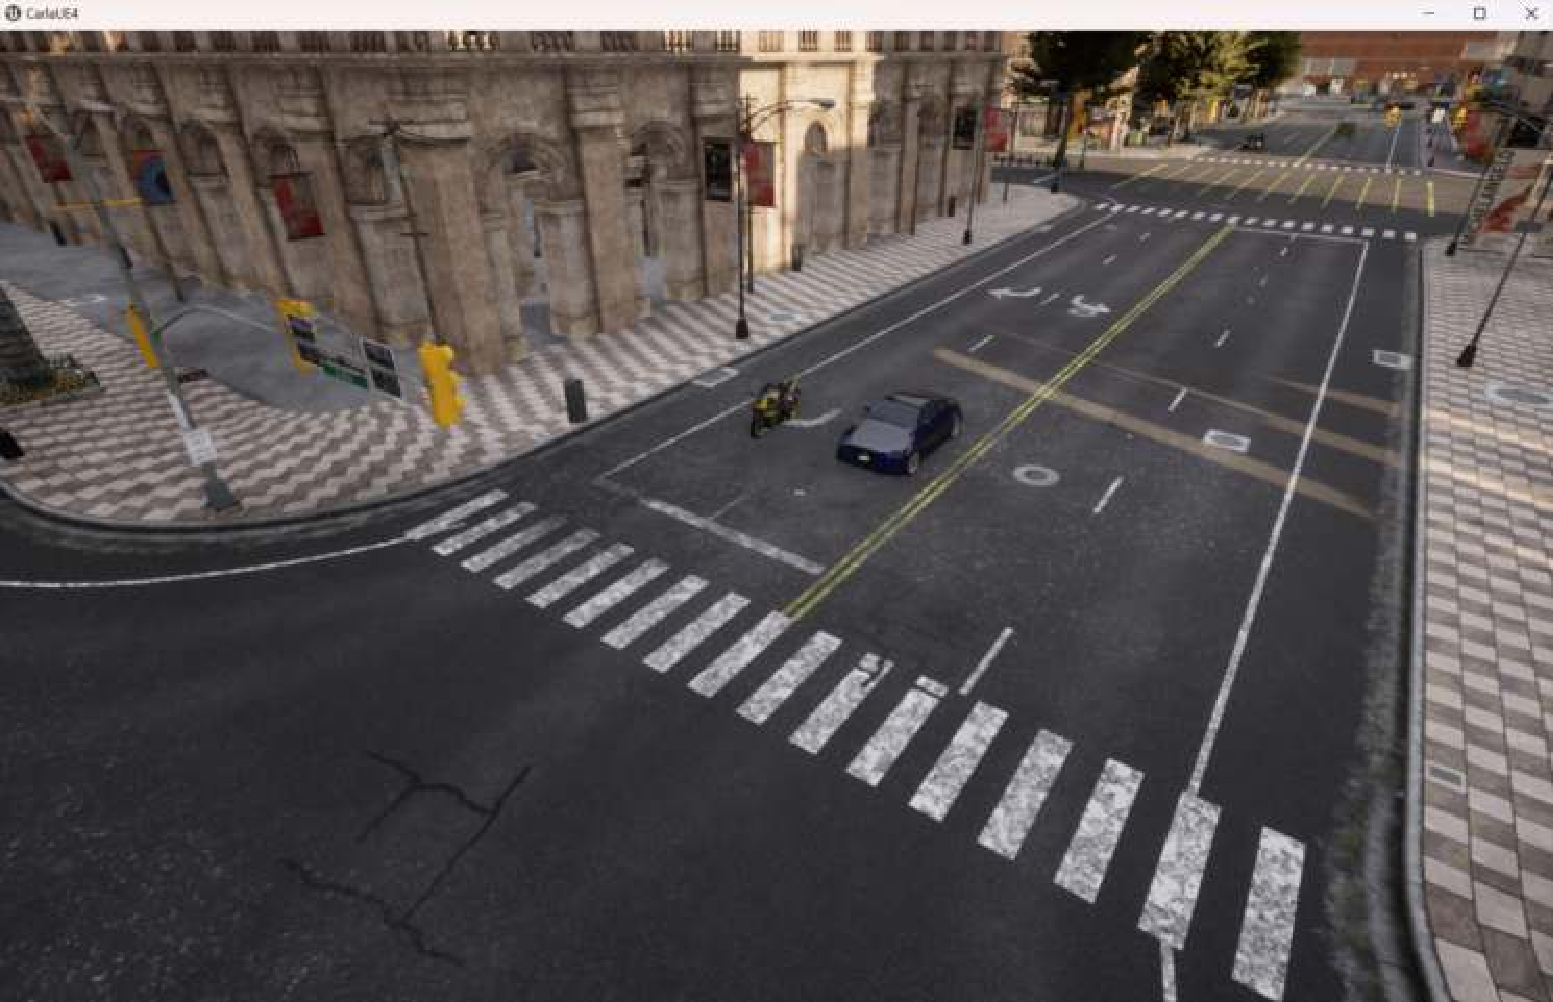
\includegraphics[width=0.7\textwidth]{"images/1.png"}
	\caption{摩托车与汽车在红绿灯前等待信号的场景截图}
	\label{fig:redlight_motorbike_car}
\end{figure}

\subsubsection{场景二:自我车辆在夜晚穿越道路}
\indent 在夜晚,一些自我车辆正在穿越道路,街道上的路灯微弱地照亮着周围环境,远处偶尔可以看到其他车辆的车灯闪烁。\\

\begin{figure}[H]
	\centering
	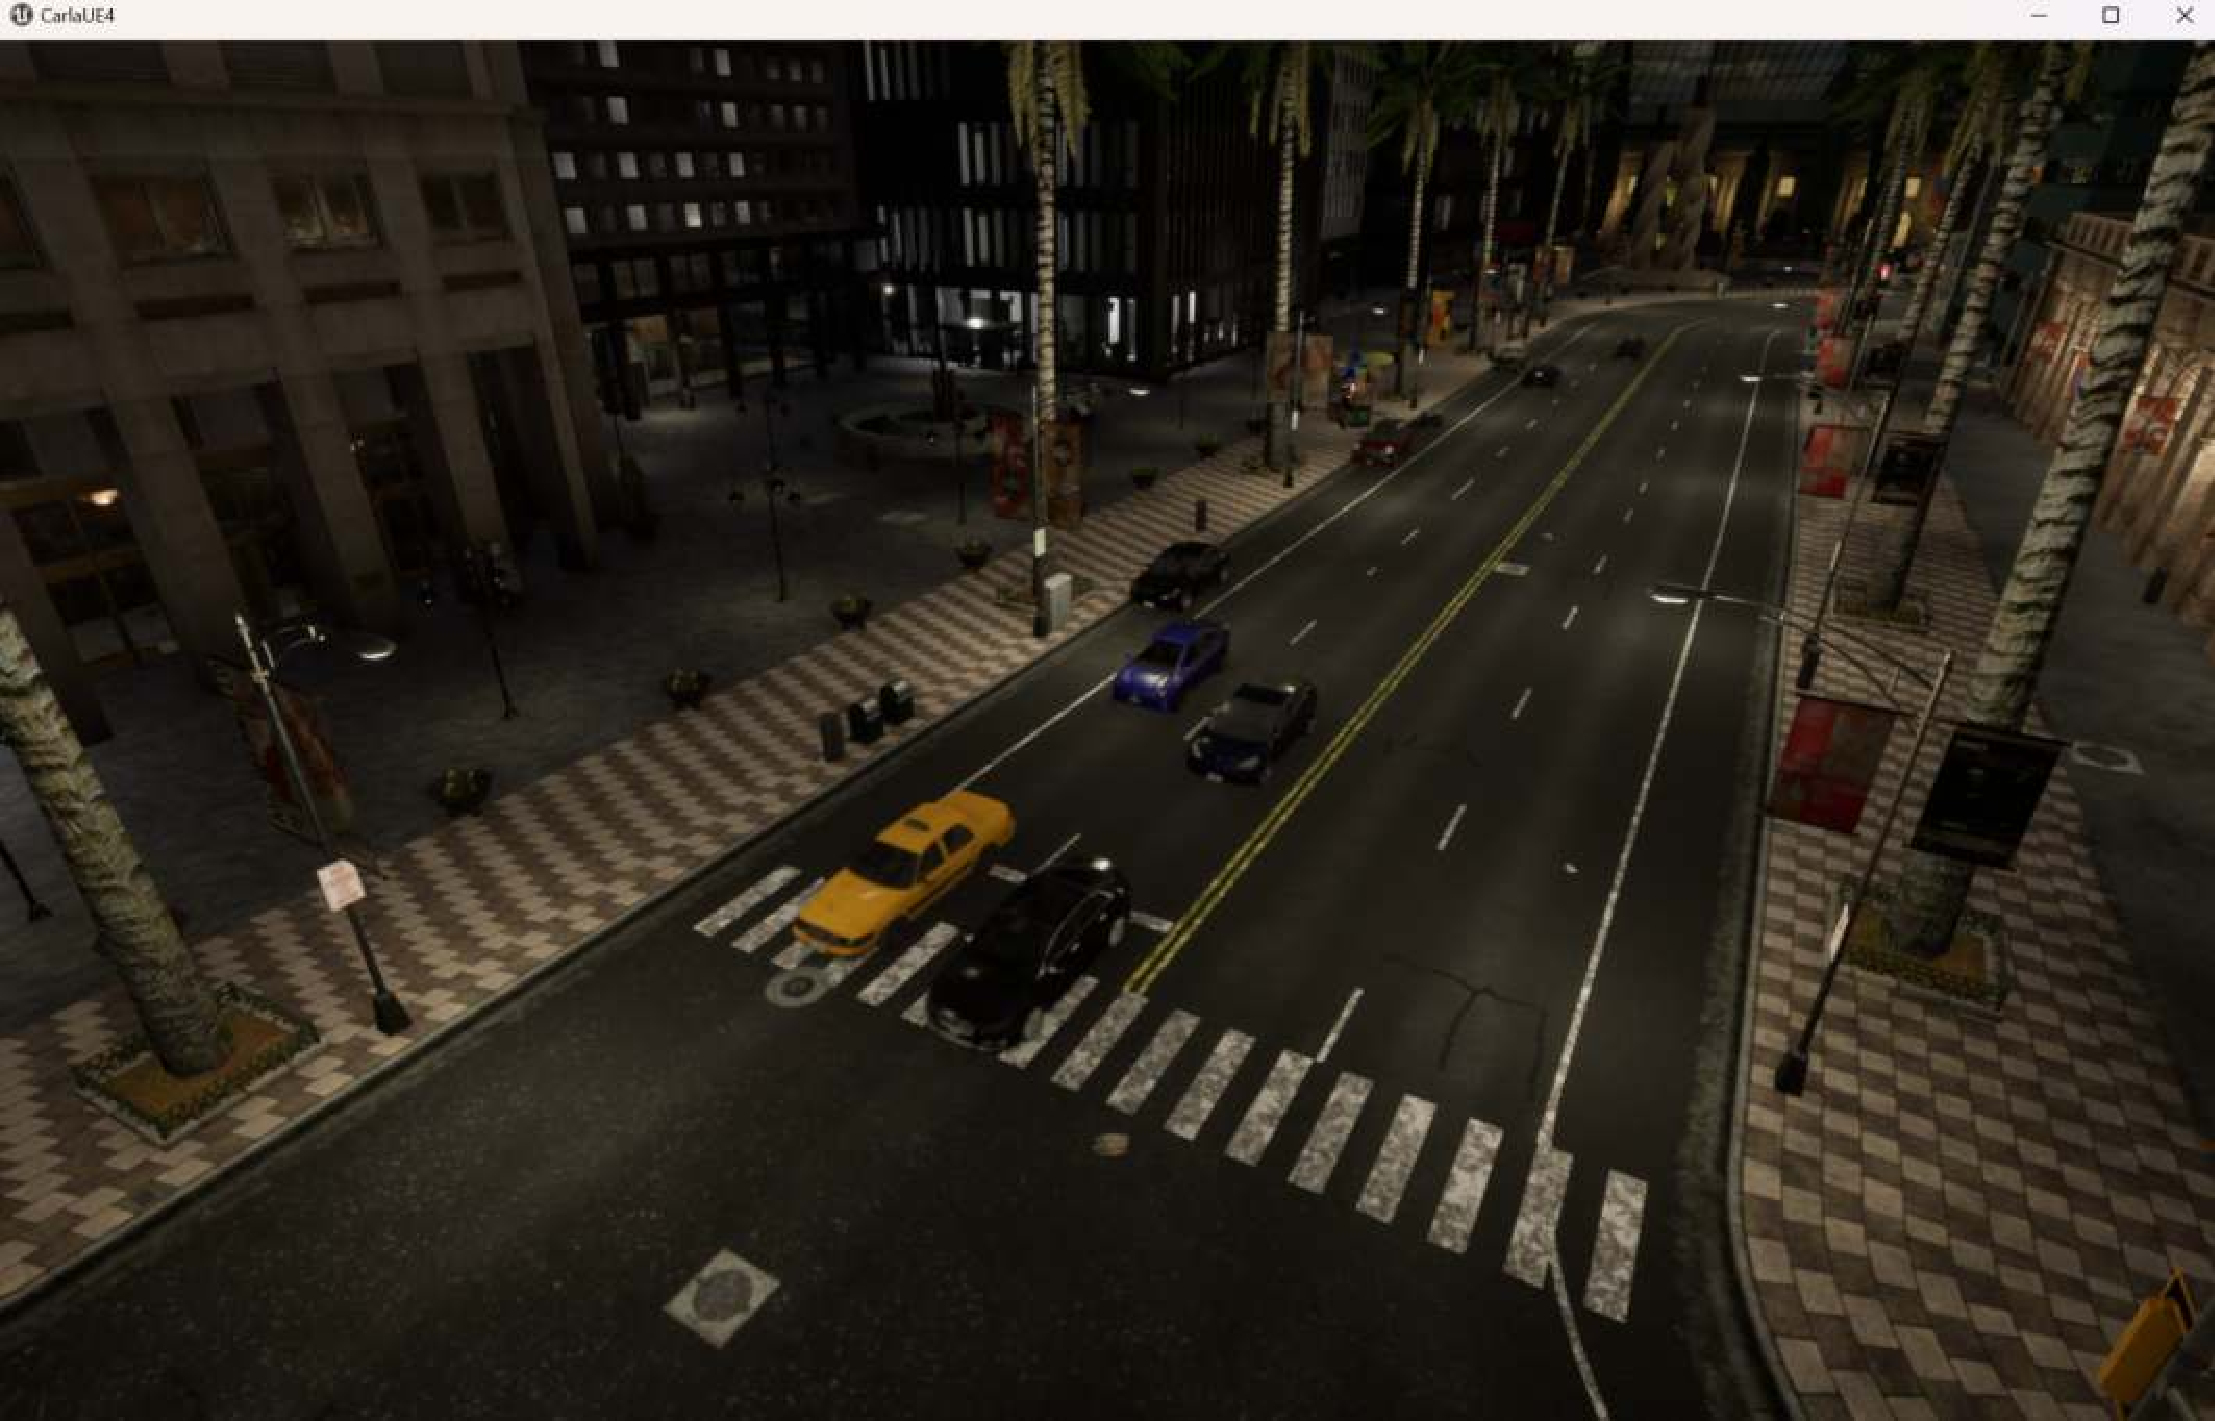
\includegraphics[width=0.7\textwidth]{"images/2.png"}
	\caption{自我车辆在夜晚穿越道路的场景截图}
	\label{fig:night_self_driving_cross}
\end{figure}

\subsubsection{场景三:自我车辆在夜晚红绿灯前等待信号}
\indent 在夜晚,一些自我车辆在红绿灯前等待信号,而在另一方向,自我车辆正在通行,车灯的光芒穿过昏暗的街道。\\

\begin{figure}[H]
	\centering
	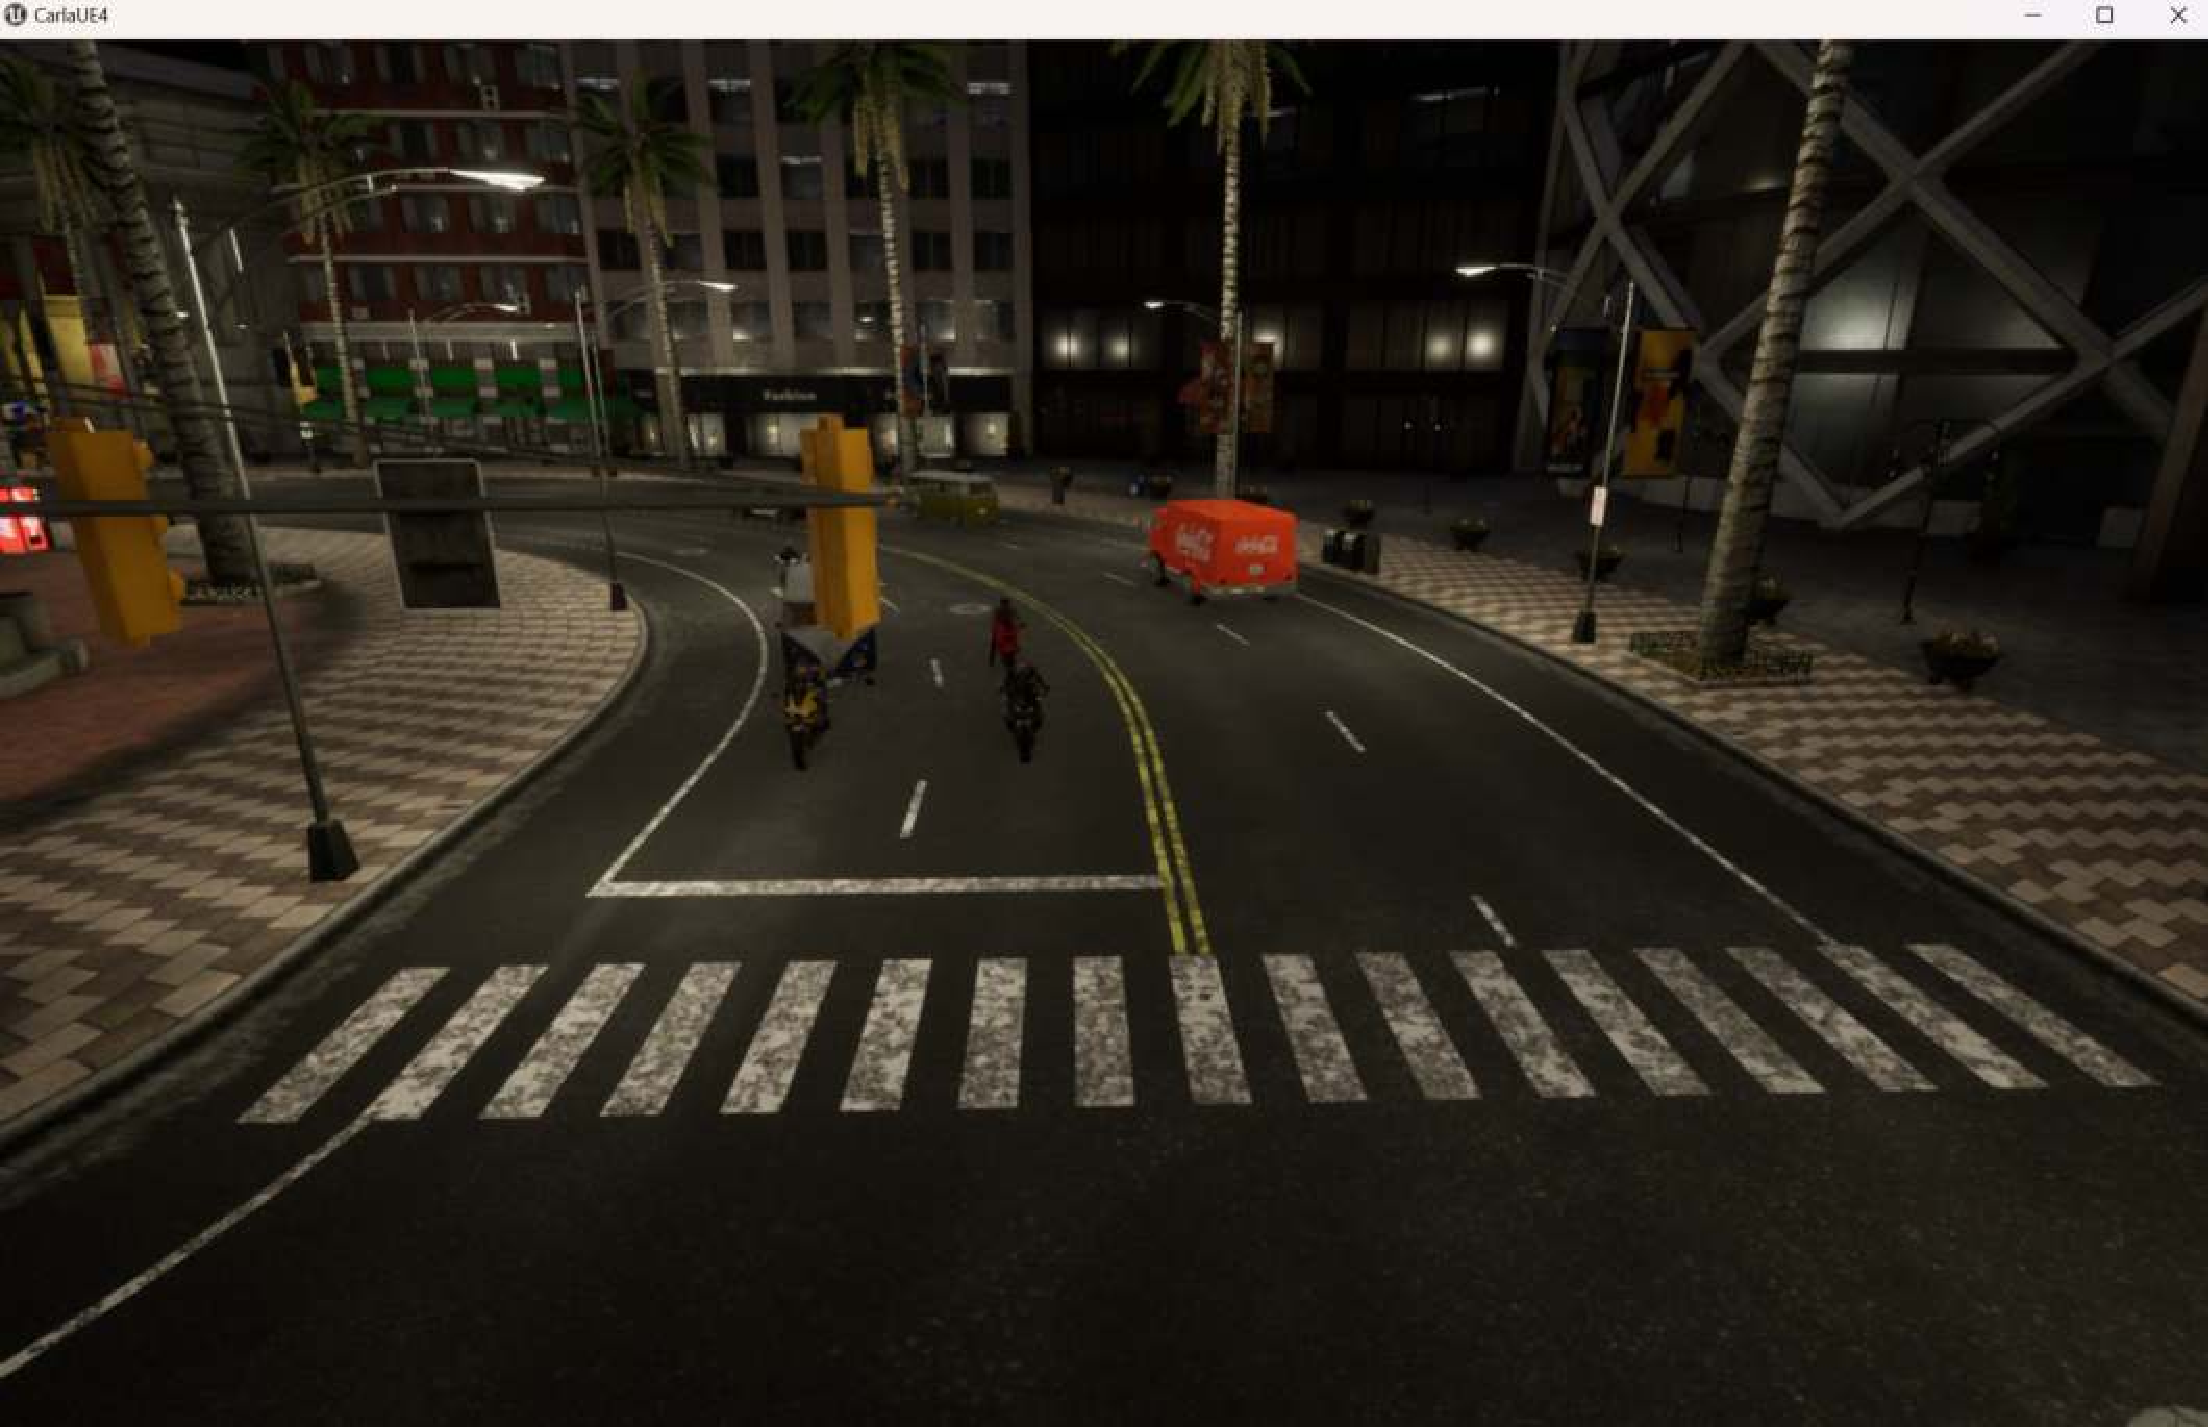
\includegraphics[width=0.7\textwidth]{"images/4.png"}
	\caption{自我车辆在夜晚红绿灯前等待信号的场景截图}
	\label{fig:night_redlight_cross}
\end{figure}

\subsubsection{场景四:行人横穿直行道路}
\indent 自我车辆在笔直的道路上行驶时,一名行人突然从右前方横穿过来,并在自我车辆接近时突然停下。\\

\begin{figure}[H]
	\centering
	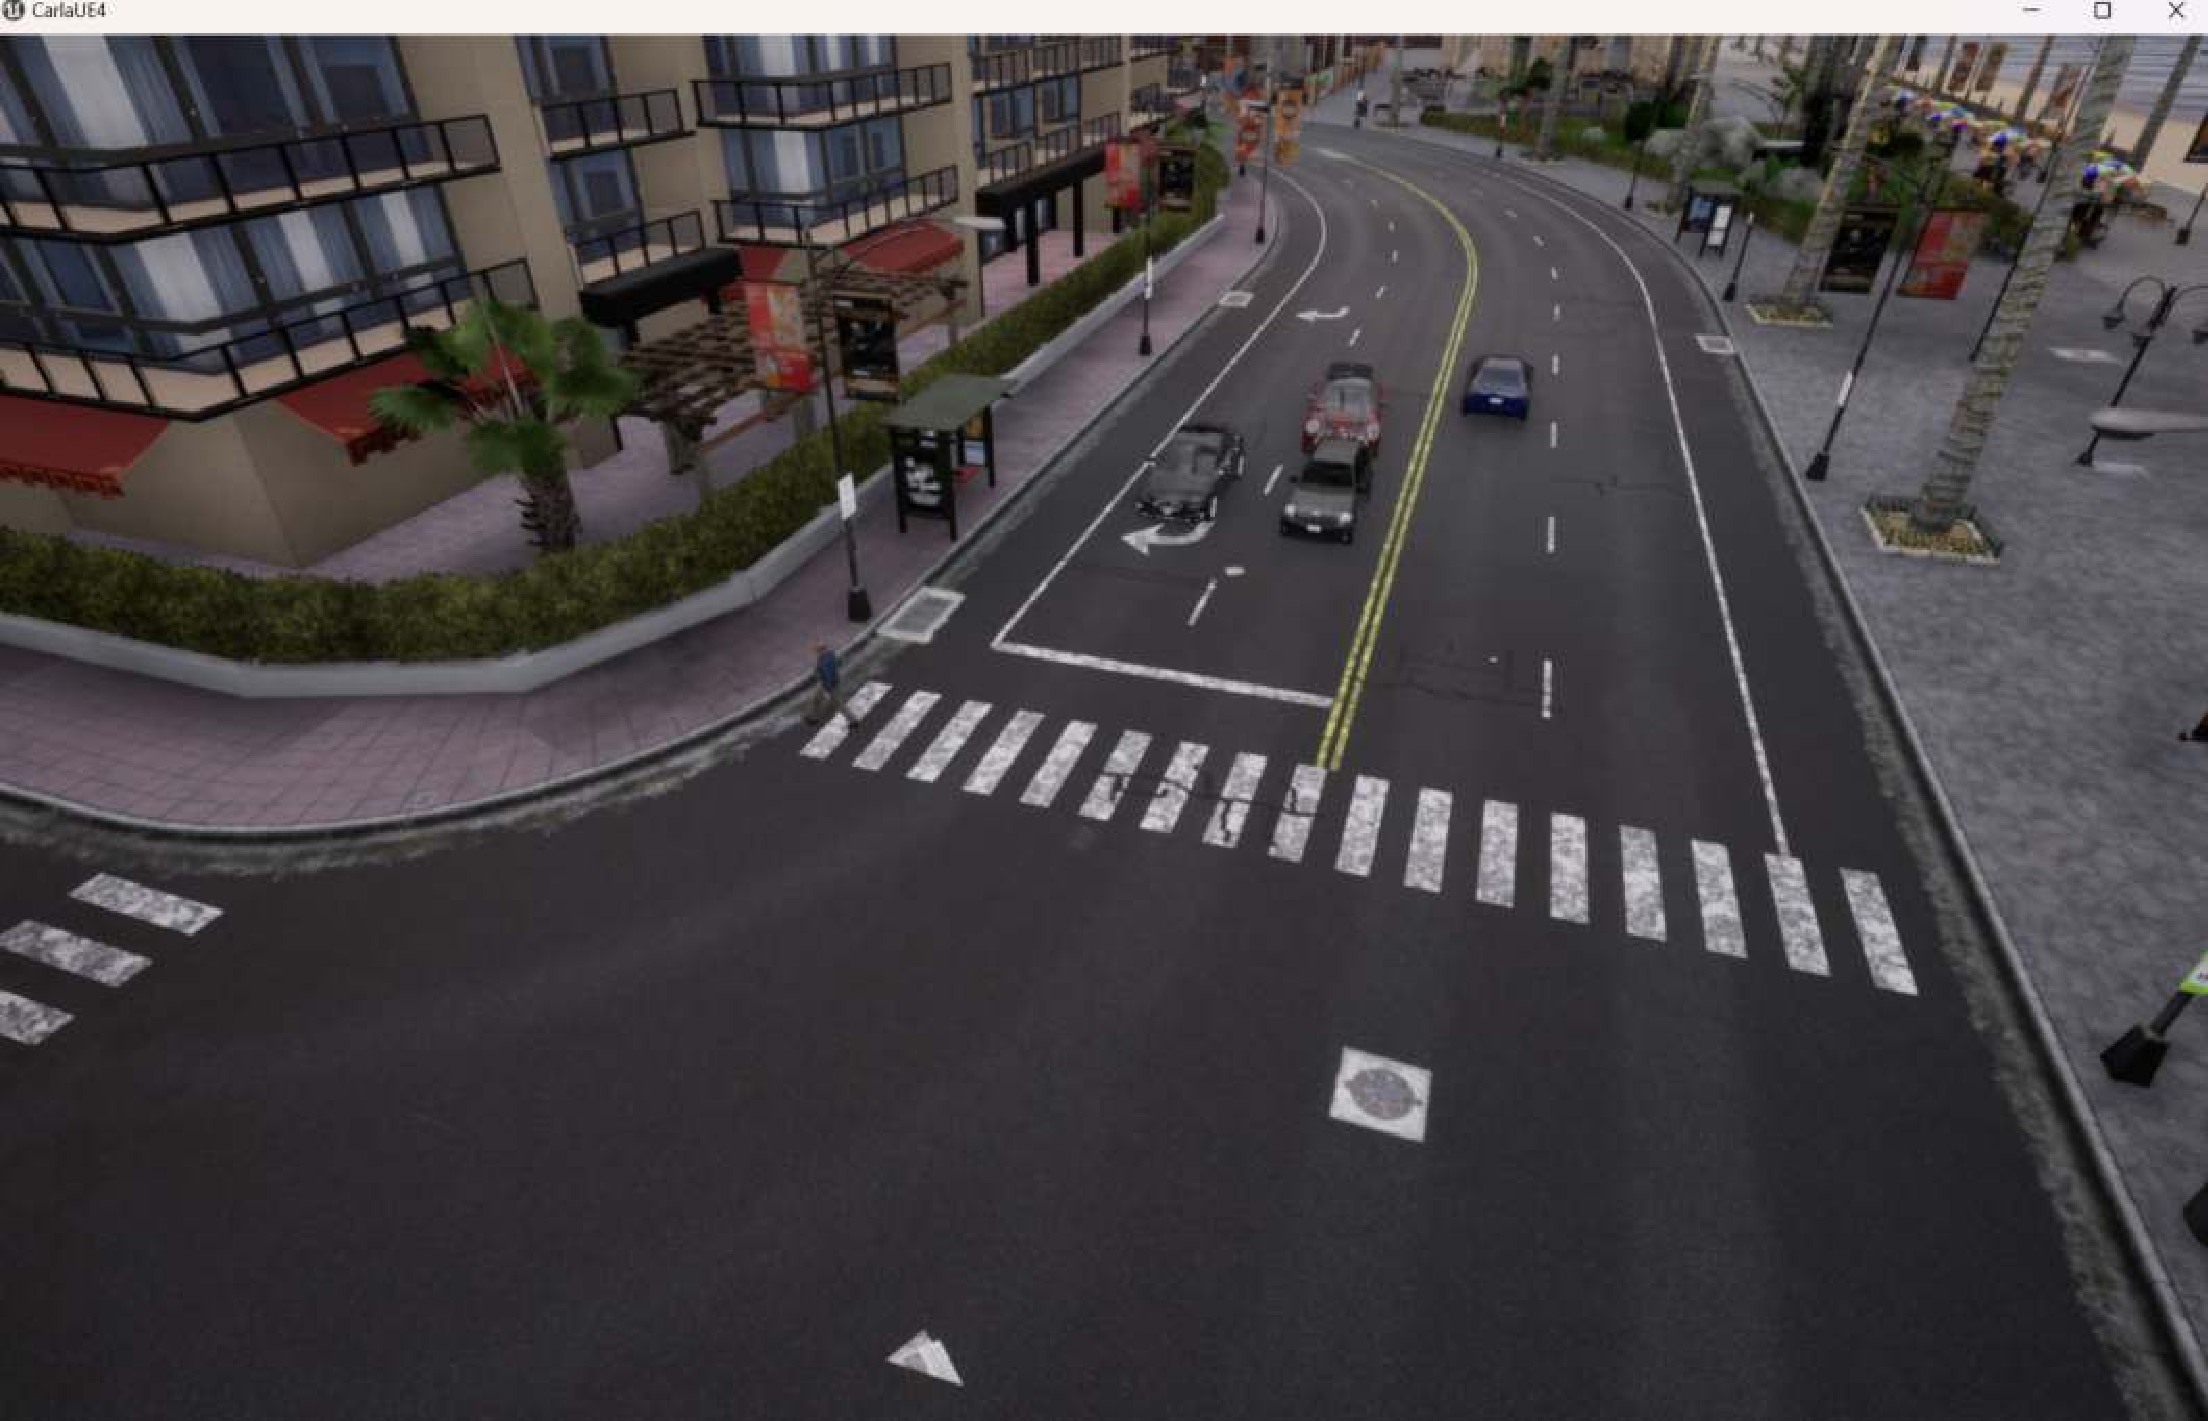
\includegraphics[width=0.7\textwidth]{"images/5.png"}
	\caption{行人横穿直行道路的场景截图}
	\label{fig:pedestrian_crossing}
\end{figure}


。




% 第五章 
\section{场景生成的量化评估}

\subsection{评估指标设计}
为客观衡量生成场景的质量,本文从以下三个维度构建评估体系:
\begin{itemize}
	\item 语义保真度(Semantic Fidelity):评估生成场景是否真实反映了输入自然语言中的核心语义要素(如参与者类型、位置关系、行为逻辑等)。使用检索式匹配与人工打分结合的方式进行评估。
	\item 场景多样性(Scene Diversity):衡量系统在不同输入下生成场景的变化程度,避免模式化输出。采用结构差异度(Structure Diversity Score)和车辆行为差异度等指标量化评估。
	\item 系统效率与响应能力(Efficiency):统计从自然语言输入到生成可视化场景的时间开销,包括语义检索、脚本生成与场景渲染的耗时。
\end{itemize}

\subsection{实验设置}
硬件配置:处理器:Intel Core i9、显卡:3060、内存:32GB

软件环境:虚拟环境:项目中使用了两个虚拟环境
\begin{enumerate}
	\item carla(Python 3.7):用于运行 CARLA 0.9.15 版本进行仿真和场景生成。
	\item chatscene(Python 3.8):用于处理与生成自然语言描述相关的任务,以及进行场景量化评估。
\end{enumerate}

依赖库:安装了必要的依赖,包括但不限于 openai, sentence\_transformers, torch 等。

输入数据:
自然语言描述:本实验使用约 20 条自然语言描述作为输入样本,这些描述用于生成自动驾驶场景。这些描述涵盖了不同的交通情况和突发事件,例如:自我车辆在红绿灯前等待信号;行人在街道上突然横穿;突然出现的障碍物等。

场景生成流程:
\begin{enumerate}
	\item 使用自然语言描述通过 ChatScene 项目生成对应的 CARLA 场景。
	\item 将生成的场景导入 CARLA 仿真环境进行验证,确保场景符合预期。
	\item 使用量化评估方法对生成的场景进行评估,分析碰撞率、响应时间、系统表现等指标。
\end{enumerate}

\subsection{评估结果与分析}
\subsubsection{5.3.1 语义保真度}
通过人工评估方式对 30 个生成场景进行语义一致性评分,得分范围为 0–5,得分越高表明语义表达越准确。结果如下:
\begin{figure}[h]
	\centering
	
\includegraphics[width=0.8\textwidth]{"images/picture1.pdf"}
	\caption{结果1}
	\label{fig:example}
\end{figure}
平均得分为 4.38,说明生成系统在语义还原方面表现优异,能够较好地捕捉自然语言中的关键词及其空间/行为语义。

\subsubsection{5.3.2 多样性分析}
在输入条件近似的情况下,系统生成了具有多样参与者布局与动作的场景。采用结构特征编码后计算场景间欧几里得距离,多样性指标(Diversity Score)平均为 0.78,说明系统具备良好的多样性能力。
此外,通过对生成的截图进行视觉对比,发现系统在车辆类型、行驶方向、光照与天气等维度的变化也具备一定随机性与可控性。

\subsubsection{5.3.3 效率分析}
系统整体生成流程的平均时间如下:
\begin{figure}[h]
	\centering
	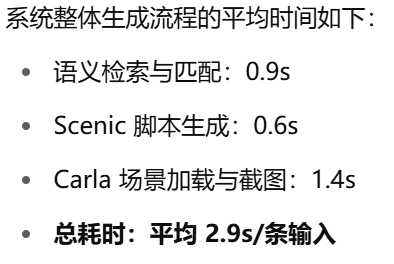
\includegraphics[width=0.5\textwidth]{"images/picture2.pdf"}
	\caption{结果2}
	\label{fig:example2}
\end{figure}
对于批量输入的处理场景,系统可维持稳定输出性能,支持实际的自动驾驶训练与测试任务需求。
\newpage
% 参考文献
\section{参考文献}
\begin{thebibliography}{99}
\bibitem{ref3}	Yasasa Abeysirigoonawardena, Florian Shkurti, and Gregory Dudek. Generating adversarial driving scenarios in high f idelity simulators. In 2019 International Conference on Robotics and Automation (ICRA), pages 8271–8277. IEEE, 2019. 3
\bibitem{ref3}	Gerrit Bagschik, Till Menzel, and Markus Maurer. Ontology based scene creation for the development of automated ve hicles. In 2018 IEEE Intelligent Vehicles Symposium (IV), pages 1813–1820. IEEE, 2018. 3 
\bibitem{ref3}	Battista Biggio, Igino Corona, Davide Maiorca, Blaine Nel son, Nedim ˇ Srndi´ c, Pavel Laskov, Giorgio Giacinto, and Fabio Roli. Evasion attacks against machine learning at test time. In Joint European conference on machine learning and knowl edge discovery in databases, pages 387–402. Springer, 2013. 1 
\bibitem{ref3}	Tom Brown, Benjamin Mann, Nick Ryder, Melanie Sub biah, Jared D Kaplan, Prafulla Dhariwal, Arvind Neelakantan, Pranav Shyam, Girish Sastry, Amanda Askell, et al. Language models are few-shot learners. Advances in neural information processing systems, 33:1877–1901, 2020. 1 
\bibitem{ref3}	Panpan Cai, Yiyuan Lee, Yuanfu Luo, and David Hsu. Sum mit: A simulator for urban driving in massive mixed traffic. In 2020 IEEE International Conference on Robotics and Au tomation (ICRA), pages 4023–4029. IEEE, 2020. 3 
\bibitem{ref3}	Yulong Cao, Chaowei Xiao, Benjamin Cyr, Yimeng Zhou, Won Park, Sara Rampazzi, Qi Alfred Chen, Kevin Fu, and Z Morley Mao. Adversarial sensor attack on lidar-based perception in autonomous driving. In Proceedings of the 2019 ACMSIGSACconference on computer and communications security, pages 2267–2281, 2019. 1 
\bibitem{ref3}	CARLA. Carla autonomous driving challenge, 2019. 3, 7 [8] Baiming Chen, Xiang Chen, Qiong Wu, and Liang Li. Ad versarial evaluation of autonomous vehicles in lane-change scenarios. IEEE transactions on intelligent transportation systems, 23(8):10333–10342, 2021. 1 
\bibitem{ref3}	Aakanksha Chowdhery, Sharan Narang, Jacob Devlin, Maarten Bosma, GauravMishra, AdamRoberts, PaulBarham, Hyung Won Chung, Charles Sutton, Sebastian Gehrmann, et al. Palm: Scaling language modeling with pathways. arXiv preprint arXiv:2204.02311, 2022. 1
\bibitem{ref3}	Scenario Runner Contributors. Carla Scenario Run ner.  
\bibitem{ref3}	Jiaxi Cui, Zongjian Li, Yang Yan, Bohua Chen, and Li Yuan. Chatlaw: Open-source legal large language model with integrated external knowledge bases. arXiv preprint arXiv:2306.16092, 2023. 2
\bibitem{ref3}	Jacob Devlin, Ming-Wei Chang, Kenton Lee, and Kristina Toutanova. Bert: Pre-training of deep bidirectional transformers for language understanding. arXiv preprint arXiv:1810.04805, 2018. 1 
\bibitem{ref3}	Wenhao Ding, Baiming Chen, Minjun Xu, and Ding Zhao. Learning to collide: An adaptive safety-critical scenarios gen erating method. In 2020 IEEE/RSJ International Conference on Intelligent Robots and Systems (IROS), pages 2243–2250. IEEE, 2020. 6 critical driving scenarios. In 2020 IEEE International Confer ence on Robotics and Automation (ICRA), pages 4314–4321. IEEE, 2020. 3
\bibitem{ref3}	Alexey Dosovitskiy, German Ros, Felipe Codevilla, Antonio Lopez, and Vladlen Koltun. Carla: An open urban driving simulator. In Conference on robot learning, pages 1–16. PMLR, 2017. 1, 2
\bibitem{ref3}	Bradley J Erickson, Panagiotis Korfiatis, Zeynettin Akkus, and Timothy L Kline. Machine learning for medical imaging. Radiographics, 37(2):505, 2017. 1
\bibitem{ref3}	Kevin Eykholt, Ivan Evtimov, Earlence Fernandes, Bo Li, Amir Rahmati, Chaowei Xiao, Atul Prakash, Tadayoshi Kohno, and Dawn Song. Robust physical-world attacks on deep learning visual classification. In Proceedings of the IEEE Conference on Computer Vision and Pattern Recogni tion, pages 1625–1634, 2018. 1 [18] Shuo Feng, Xintao Yan, Haowei Sun, Yiheng Feng, and Henry X Liu. Intelligent driving intelligence test for au tonomous vehicles with naturalistic and adversarial environ ment. Nature communications, 12(1):748, 2021. 1 
\bibitem{ref3}	Daniel J Fremont, Tommaso Dreossi, Shromona Ghosh, Xi angyu Yue, Alberto L Sangiovanni-Vincentelli, and Sanjit A Seshia. Scenic: a language for scenario specification and scene generation. In Proceedings of the 40th ACM SIGPLAN Conference on Programming Language Design and Imple mentation, pages 63–78, 2019. 2, 4 
\bibitem{ref3}	Daniel J Fremont, Edward Kim, TommasoDreossi, Shromona Ghosh, Xiangyu Yue, Alberto L Sangiovanni-Vincentelli, and Sanjit A Seshia. Scenic: A language for scenario specification and data generation. Machine Learning, pages 1–45, 2022. 2, 4
\bibitem{ref3}	Daocheng Fu, Xin Li, Licheng Wen, Min Dou, Pinlong Cai, Botian Shi, and Yu Qiao. Drive like a human: Rethinking au tonomous driving with large language models. arXiv preprint arXiv:2307.07162, 2023. 3 
\bibitem{ref3}	Scott Fujimoto, Herke van Hoof, and David Meger. Address ing function approximation error in actor-critic methods. In Proceedings of the 35th International Conference on Machine Learning, pages 1587–1596. PMLR, 2018. 6 
\bibitem{ref3}	Tuomas Haarnoja, Aurick Zhou, Pieter Abbeel, and Sergey Levine. Soft actor-critic: Off-policy maximum entropy deep reinforcement learning with a stochastic actor. In Proceedings of the 35th International Conference on Machine Learning, pages 1861–1870. PMLR, 2018. 6
\bibitem{ref3}	Kaiming He, Xiangyu Zhang, Shaoqing Ren, and Jian Sun. Deep residual learning for image recognition. In Proceed ings of the IEEE conference on computer vision and pattern recognition, pages 770–778, 2016. 1 
\bibitem{ref3}	Jeff Johnson, Matthijs Douze, and Herv´ e J´ egou. Billion-scale similarity search with GPUs. IEEE Transactions on Big Data, 7(3):535–547, 2019. 5 
\bibitem{ref3}	Enkelejda Kasneci, Kathrin Seßler, Stefan K¨ uchemann, Maria Bannert, Daryna Dementieva, Frank Fischer, Urs Gasser, Georg Groh, Stephan G¨unnemann, Eyke H¨ullermeier, et al. Chatgpt for good? on opportunities and challenges of large 15467 language models for education. Learning and individual differences, 103:102274, 2023. 1 
\bibitem{ref3}	Moritz Klischat, Edmond Irani Liu, Fabian Holtke, and Matthias Althoff. Scenario factory: Creating safety-critical traffic scenarios for automated vehicles. In 2020 IEEE 23rd International Conference on Intelligent Transportation Sys tems (ITSC), pages 1–7. IEEE, 2020. 3 
\bibitem{ref3}	Zelun Kong, Junfeng Guo, Ang Li, and Cong Liu. Physgan: Generating physical-world-resilient adversarial examples for autonomous driving. In Proceedings of the IEEE/CVF Con ference on Computer Vision and Pattern Recognition, pages 14254–14263, 2020. 1
\bibitem{ref3}	Ritchie Lee, Mykel J Kochenderfer, Ole J Mengshoel, Guil laume P Brat, and Michael P Owen. Adaptive stress testing of airborne collision avoidance systems. In 2015 IEEE/AIAA 34th Digital Avionics Systems Conference (DASC), pages 6C2–1. IEEE, 2015. 3 
\bibitem{ref3}	Wassim G Najm, John D Smith, Mikio Yanagisawa, et al. Pre-crash scenario typology for crash avoidance research. Technical report, United States. National Highway Traffic Safety Administration, 2007. 7 
\bibitem{ref3}	Jianmo Ni, Gustavo Hernandez Abrego, Noah Constant, Ji Ma, Keith Hall, Daniel Cer, and Yinfei Yang. Sentence t5: Scalable sentence encoders from pre-trained text-to-text models. In Findings of the Association for Computational Linguistics: ACL 2022, pages 1864–1874, 2022. 5
\bibitem{ref3}	Erik Nijkamp, Bo Pang, Hiroaki Hayashi, Lifu Tu, Huan Wang, Yingbo Zhou, Silvio Savarese, and Caiming Xiong. Codegen: An open large language model for code with multi turn program synthesis. In The Eleventh International Con ference on Learning Representations, 2022. 2 
\bibitem{ref3}	Aayush Prakash, Shaad Boochoon, Mark Brophy, David Acuna, Eric Cameracci, Gavriel State, Omer Shapira, and Stan Birchfield. Structured domain randomization: Bridging the reality gap by context-aware synthetic data. In 2019 In ternational Conference on Robotics and Automation (ICRA), pages 7249–7255. IEEE, 2019. 3
\bibitem{ref3}	Davis Rempe, Jonah Philion, Leonidas J Guibas, Sanja Fi dler, and Or Litany. Generating useful accident-prone driv ing scenarios via a learned traffic prior. In Proceedings of the IEEE/CVF Conference on Computer Vision and Pattern Recognition, pages 17305–17315, 2022. 3
\bibitem{ref3}	Elias Rocklage, Heiko Kraft, Abdullah Karatas, and J¨org Seewig. Automated scenario generation for regression testing of autonomous vehicles. In 2017 ieee 20th international conference on intelligent transportation systems (itsc), pages 476–483. IEEE, 2017. 3 
\bibitem{ref3}	John M Scanlon, Kristofer D Kusano, Tom Daniel, Christo pher Alderson, Alexander Ogle, and Trent Victor. Waymo sim ulated driving behavior in reconstructed fatal crashes within an autonomous vehicle operating domain. Accident Analysis Prevention, 163:106454, 2021. 3 
\bibitem{ref3}	John Schulman, Filip Wolski, Prafulla Dhariwal, Alec Rad ford, and Oleg Klimov. Proximal policy optimization algo rithms. arXiv preprint arXiv:1707.06347, 2017. 6 [38] Karan Singhal, Shekoofeh Azizi, Tao Tu, S Sara Mahdavi, Jason Wei, Hyung Won Chung, Nathan Scales, Ajay Tan wani, Heather Cole-Lewis, Stephen Pfohl, et al. Large lan guage models encode clinical knowledge. arXiv preprint arXiv:2212.13138, 2022. 2 
\bibitem{ref3}	Christian Szegedy, Wojciech Zaremba, Ilya Sutskever, Joan Bruna, Dumitru Erhan, Ian Goodfellow, and Rob Fergus. Intriguing properties of neural networks. In 2nd International Conference on Learning Representations, ICLR 2014, 2014. 1 
\bibitem{ref3}	Shuhan Tan, Boris Ivanovic, Xinshuo Weng, Marco Pavone, and Philipp Kraehenbuehl. Language conditioned traffic gen eration. In Conference on Robot Learning, pages 2714–2752. PMLR, 2023. 3 
\bibitem{ref3}	Hugo Touvron, Thibaut Lavril, Gautier Izacard, Xavier Mar tinet, Marie-Anne Lachaux, Timoth´ee Lacroix, Baptiste Rozi`ere, Naman Goyal, Eric Hambro, Faisal Azhar, et al. Llama: Openandefficient foundation language models. arXiv preprint arXiv:2302.13971, 2023. 1 
\bibitem{ref3}	Robin van der Made, Martijn Tideman, Ulrich Lages, Roman Katz, and Martin Spencer. Automated generation of virtual driving scenarios from test drive data. In 24th International Technical Conference on the Enhanced Safety of Vehicles (ESV) National Highway Traffic Safety Administration, num ber 15-0268, 2015. 3
\bibitem{ref3}	Akifumi Wachi. Failure-scenario maker for rule-based agent using multi-agent adversarial reinforcement learning and its application to autonomous driving. In International Joint Conference on Artificial Intelligence. International Joint Con ferences on Artificial Intelligence, 2019. 1
\bibitem{ref3}	Jingkang Wang, Ava Pun, James Tu, Sivabalan Manivasagam, Abbas Sadat, Sergio Casas, Mengye Ren, and Raquel Urtasun. Advsim: Generating safety-critical scenarios for self-driving vehicles. In Proceedings of the IEEE/CVF Conference on Computer Vision and Pattern Recognition, pages 9909–9918, 2021. 6
\bibitem{ref3}	Shijie Wu, Ozan Irsoy, Steven Lu, Vadim Dabravolski, Mark Dredze, Sebastian Gehrmann, Prabhanjan Kambadur, David Rosenberg, and Gideon Mann. Bloomberggpt: A large lan guage model for finance. arXiv preprint arXiv:2303.17564, 2023. 2
\bibitem{ref3}	Chejian Xu, Wenhao Ding, Weijie Lyu, Zuxin Liu, Shuai Wang, Yihan He, Hanjiang Hu, Ding Zhao, and Bo Li. Safebench: A benchmarking platform for safety evaluation of autonomous vehicles. Advances in Neural Information Processing Systems, 35:25667–25682, 2022. 2, 6, 12 
\bibitem{ref3}	Zhenhua Xu, Yujia Zhang, Enze Xie, Zhen Zhao, Yong Guo, Kenneth KY Wong, Zhenguo Li, and Hengshuang Zhao. Drivegpt4: Interpretable end-to-end autonomous driving via large language model. arXiv preprint arXiv:2310.01412, 2023. 3 
\bibitem{ref3}	Zhenpei Yang, Yuning Chai, Dragomir Anguelov, Yin Zhou, Pei Sun, Dumitru Erhan, Sean Rafferty, and Henrik Kret zschmar. Surfelgan: Synthesizing realistic sensor data for autonomous driving. In Proceedings of the IEEE/CVF Con ference on Computer Vision and Pattern Recognition, pages 11118–11127, 2020. 3
\bibitem{ref3}	Shunyu Yao, Jeffrey Zhao, Dian Yu, Nan Du, Izhak Shafran, Karthik R Narasimhan, and Yuan Cao. React: Synergizing 15468 reasoning and acting in language models. In The Eleventh International Conference on Learning Representations, 2022. 3 
\bibitem{ref3}	Linrui Zhang, Zhenghao Peng, Quanyi Li, and Bolei Zhou. Cat: Closed-loop adversarial training for safe end-to-end driving. In Conference on Robot Learning, pages 2357–2372. PMLR, 2023. 3
\bibitem{ref3}	Qingzhao Zhang, Shengtuo Hu, Jiachen Sun, Qi Alfred Chen, and Z Morley Mao. On adversarial robustness of trajec tory prediction for autonomous vehicles. arXiv preprint arXiv:2201.05057, 2022. 6 
\bibitem{ref3}	Lianmin Zheng, Wei-Lin Chiang, Ying Sheng, Siyuan Zhuang, Zhanghao Wu, YonghaoZhuang, Zi Lin, Zhuohan Li, Dacheng Li, Eric Xing, et al. Judging llm-as-a-judge with mt bench and chatbot arena. arXiv preprint arXiv:2306.05685, 2023. 1 
\bibitem{ref3}	Ziyuan Zhong, Davis Rempe, Yuxiao Chen, Boris Ivanovic, Yulong Cao, Danfei Xu, Marco Pavone, and Baishakhi Ray. Language-guided traffic simulation via scene-level diffusion. arXiv preprint arXiv:2306.06344, 2023. 3
\bibitem{ref3}	赵祥模,童星,穆柯楠,等.面向自动驾驶汽车测试需求的关键场景要素提取方法[J/OL].中国公路学报,1-15[2025-04-21].http://kns.cnki.net/kcms/detail/61.1313.U.20250418.1427.006.html.
\bibitem{ref3}	杜德慧,叶振,郑成行,等.面向自动驾驶系统的场景建模及边缘关键场景生成[J/OL].软件学报,1-19[2025-04-21].https://doi.org/10.13328/j.cnki.jos.007348.
\bibitem{ref3}	彭海洋,计卫星,刘法旺.基于多节点仿真的自动驾驶场景数据保护方法[J/OL].汽车工程学报,1-12[2025-04-21].http://kns.cnki.net/kcms/detail/50.1206.U.20250402.1146.002.html.
\bibitem{ref3}	方虹苏,常城,石鑫雨,等.自动驾驶场景中YOLO目标检测算法的应用研究[J].汽车实用技术,2025,50(06):65-74.DOI:10.16638/j.cnki.1671-7988.2025.006.011.
\bibitem{ref3}	伍毅平,张鸿鹏,陈家源,等.考虑场景与驾驶风格差异的出租车驾驶人驾驶行为特性分析[J/OL].武汉理工大学学报(交通科学与工程版),1-7[2025-04-21].http://kns.cnki.net/kcms/detail/42.1824.U.20250319.1733.016.html.
\bibitem{ref3}	宋华,吴贤静,吴琼,等.基于自然驾驶数据构建仿真测试变道切入场景库的方法[J/OL].汽车工程学报,1-12[2025-04-21].http://kns.cnki.net/kcms/detail/50.1206.u.20250228.1707.002.html.
\bibitem{ref3}	王润民,何佳浚,冯皓.跟随自动驾驶汽车行驶场景下的驾驶人行为分析与建模[J/OL].计算机工程与应用,1-12[2025-04-21].http://kns.cnki.net/kcms/detail/11.2127.TP.20250225.0933.002.html.
\bibitem{ref3}	吕叶祥子,蒋渊德,宋家乐,等.基于神经渲染的自动驾驶场景解耦表征与感知数据生成[J/OL].汽车工程学报,1-13[2025-04-21].http://kns.cnki.net/kcms/detail/50.1206.U.20250219.1136.004.html.
\bibitem{ref3}	武彪,任洪泽,郑联庆,等.基于自然驾驶行为的智能驾驶复杂场景构建方法[J].华南理工大学学报(自然科学版),2025,53(02):38-47.
\bibitem{ref3}	顾同成,徐东伟,孙成巨.无人驾驶深度强化学习决策模型性能评测方法综述[J/OL].计算机工程与应用,1-42[2025-04-21].http://kns.cnki.net/kcms/detail/11.2127.TP.20250414.1614.026.html.
\bibitem{ref3}	朱宇,徐志刚,赵祥模,等.基于TsGAN的自动驾驶汽车高速公路变道切入测试场景自动生成算法[J].华南理工大学学报(自然科学版),2024,52(08):76-88.

\end{thebibliography}

\end{document}




